\section{Discussion}

\begin{marginfigure}
    \centering 
    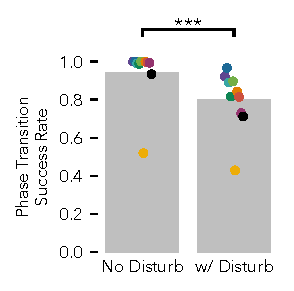
\includegraphics[width=\textwidth]{phase_success}
    \caption{Fraction of steps for which impedance control successfully
    transitions through all three stance phases. Introduction of gait
    disturbances significantly decreases the transition success rate. Grey bars
    show the mean success rate across all users. Statistical significance
    assessed by Welch's $t$-test. $***$:~$p <
    0.001$.}\label{fig:treadmill_exp_phase_success}
\end{marginfigure}
One possible reason for the increase in torso pitch variability for the
impedance controller in the disturbance case could be that the impedance
controller failed to transition to the third, ``push off'', phase of gait
significantly more often when gait was disturbed (see
\cref{fig:treadmill_exp_phase_success}). As shown in
\cref{fig:treadmill_imp_fit} if the impedance control remains in phase 2 at the
nd of gait.
